\section{Dummy\-Engine Class Reference}
\label{classDummyEngine}\index{DummyEngine@{DummyEngine}}
Inheritance diagram for Dummy\-Engine:\begin{figure}[H]
\begin{center}
\leavevmode
\includegraphics[width=86pt]{classDummyEngine__inherit__graph}
\end{center}
\end{figure}
Collaboration diagram for Dummy\-Engine:\begin{figure}[H]
\begin{center}
\leavevmode
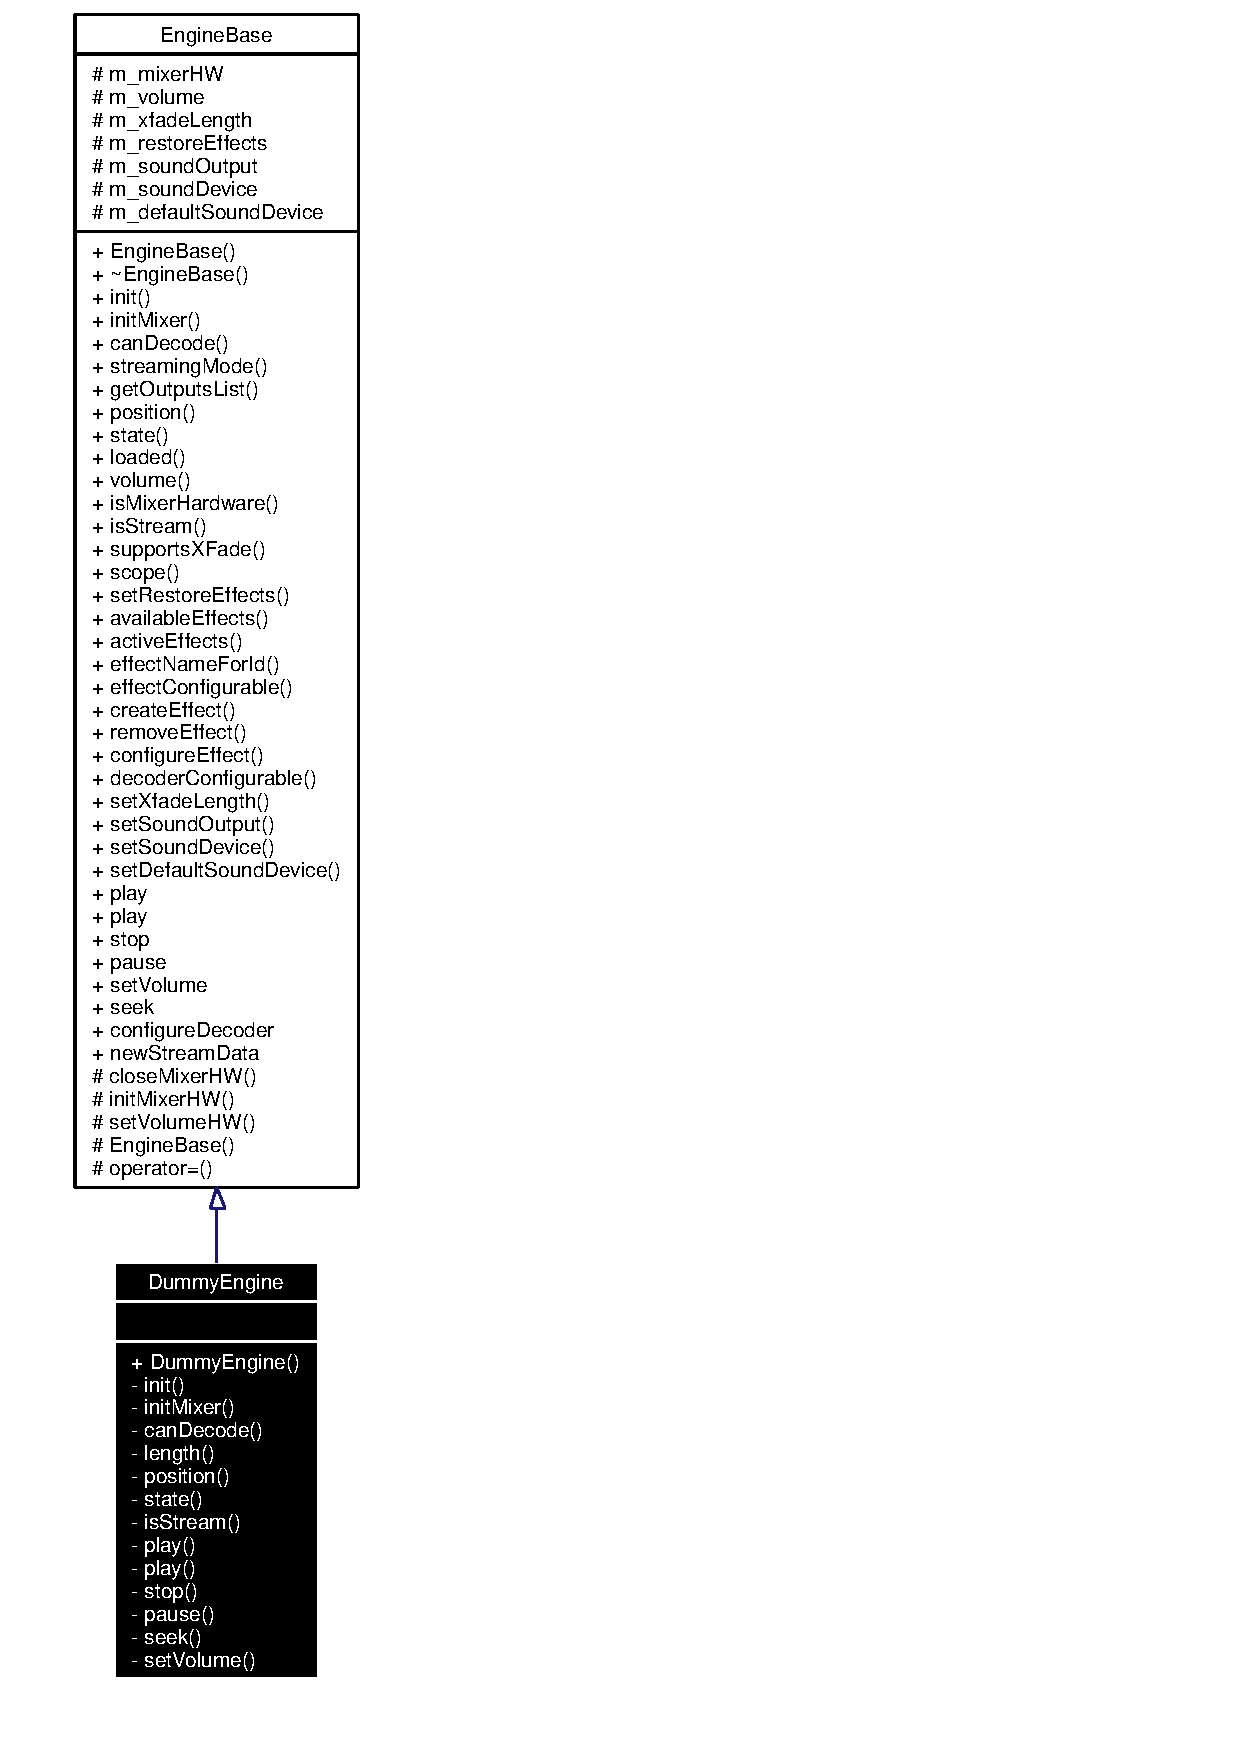
\includegraphics[width=86pt]{classDummyEngine__coll__graph}
\end{center}
\end{figure}
\subsection*{Public Types}
\begin{CompactItemize}
\item 
enum {\bf Engine\-State} \{ {\bf Empty}, 
{\bf Idle}, 
{\bf Playing}, 
{\bf Paused}
 \}
\item 
enum {\bf Streaming\-Mode} \{ {\bf Socket}, 
{\bf Signal}, 
{\bf No\-Streaming}
 \}
\end{CompactItemize}
\subsection*{Public Slots}
\begin{CompactItemize}
\item 
virtual void {\bf configure\-Decoder} ()
\item 
virtual void {\bf new\-Stream\-Data} (char $\ast$, int)
\end{CompactItemize}
\subsection*{Signals}
\begin{CompactItemize}
\item 
void {\bf end\-Of\-Track} ()
\item 
void {\bf stopped} ()
\end{CompactItemize}
\subsection*{Public Member Functions}
\begin{CompactItemize}
\item 
{\bf Dummy\-Engine} ()
\item 
virtual {\bf Streaming\-Mode} {\bf streaming\-Mode} ()
\item 
virtual QString\-List {\bf get\-Outputs\-List} ()
\item 
bool {\bf loaded} ()
\item 
int {\bf volume} () const 
\item 
bool {\bf is\-Mixer\-Hardware} () const 
\item 
virtual bool {\bf supports\-XFade} () const 
\item 
virtual std::vector$<$ float $>$ $\ast$ {\bf scope} ()
\item 
void {\bf set\-Restore\-Effects} (bool yes)
\item 
virtual QString\-List {\bf available\-Effects} () const 
\item 
virtual std::vector$<$ long $>$ {\bf active\-Effects} () const 
\item 
virtual QString {\bf effect\-Name\-For\-Id} (long) const 
\item 
virtual bool {\bf effect\-Configurable} (long) const 
\item 
virtual long {\bf create\-Effect} (const QString \&)
\item 
virtual void {\bf remove\-Effect} (long)
\item 
virtual void {\bf configure\-Effect} (long)
\item 
virtual bool {\bf decoder\-Configurable} () const 
\item 
virtual void {\bf set\-Xfade\-Length} (int ms)
\item 
virtual void {\bf set\-Sound\-Output} (const QString \&output)
\item 
virtual void {\bf set\-Sound\-Device} (const QString \&device)
\item 
virtual void {\bf set\-Default\-Sound\-Device} (bool is\-Default)
\end{CompactItemize}
\subsection*{Protected Member Functions}
\begin{CompactItemize}
\item 
void {\bf close\-Mixer\-HW} ()
\item 
bool {\bf init\-Mixer\-HW} ()
\item 
void {\bf set\-Volume\-HW} (int percent)
\end{CompactItemize}
\subsection*{Protected Attributes}
\begin{CompactItemize}
\item 
int {\bf m\_\-mixer\-HW}
\item 
int {\bf m\_\-volume}
\item 
int {\bf m\_\-xfade\-Length}
\item 
bool {\bf m\_\-restore\-Effects}
\item 
QString {\bf m\_\-sound\-Output}
\item 
QString {\bf m\_\-sound\-Device}
\item 
bool {\bf m\_\-default\-Sound\-Device}
\end{CompactItemize}
\subsection*{Private Member Functions}
\begin{CompactItemize}
\item 
virtual void {\bf init} (bool \&, int, bool)
\item 
virtual bool {\bf init\-Mixer} (bool)
\item 
virtual bool {\bf can\-Decode} (const KURL \&, mode\_\-t, mode\_\-t)
\item 
virtual long {\bf length} () const 
\item 
virtual long {\bf position} () const 
\item 
virtual {\bf Engine\-State} {\bf state} () const 
\item 
virtual bool {\bf is\-Stream} () const 
\item 
virtual void {\bf play} (const KURL \&)
\item 
virtual void {\bf play} ()
\item 
virtual void {\bf stop} ()
\item 
virtual void {\bf pause} ()
\item 
virtual void {\bf seek} (long)
\item 
virtual void {\bf set\-Volume} (int v)
\end{CompactItemize}


\subsection{Member Enumeration Documentation}
\index{DummyEngine@{Dummy\-Engine}!EngineState@{EngineState}}
\index{EngineState@{EngineState}!DummyEngine@{Dummy\-Engine}}
\subsubsection{\setlength{\rightskip}{0pt plus 5cm}enum {\bf Engine\-Base::Engine\-State}\hspace{0.3cm}{\tt  [inherited]}}\label{classEngineBase_EngineBasew7}


\begin{Desc}
\item[Enumeration values: ]\par
\begin{description}
\index{Empty@{Empty}!DummyEngine@{DummyEngine}}\index{DummyEngine@{DummyEngine}!Empty@{Empty}}\item[{\em 
Empty\label{classEngineBase_EngineBasew7EngineBasew0}
}]\index{Idle@{Idle}!DummyEngine@{DummyEngine}}\index{DummyEngine@{DummyEngine}!Idle@{Idle}}\item[{\em 
Idle\label{classEngineBase_EngineBasew7EngineBasew1}
}]\index{Playing@{Playing}!DummyEngine@{DummyEngine}}\index{DummyEngine@{DummyEngine}!Playing@{Playing}}\item[{\em 
Playing\label{classEngineBase_EngineBasew7EngineBasew2}
}]\index{Paused@{Paused}!DummyEngine@{DummyEngine}}\index{DummyEngine@{DummyEngine}!Paused@{Paused}}\item[{\em 
Paused\label{classEngineBase_EngineBasew7EngineBasew3}
}]\end{description}
\end{Desc}



Definition at line 43 of file enginebase.h.



\footnotesize\begin{verbatim}43 { Empty, Idle, Playing, Paused };
\end{verbatim}\normalsize 
\index{DummyEngine@{Dummy\-Engine}!StreamingMode@{StreamingMode}}
\index{StreamingMode@{StreamingMode}!DummyEngine@{Dummy\-Engine}}
\subsubsection{\setlength{\rightskip}{0pt plus 5cm}enum {\bf Engine\-Base::Streaming\-Mode}\hspace{0.3cm}{\tt  [inherited]}}\label{classEngineBase_EngineBasew8}


\begin{Desc}
\item[Enumeration values: ]\par
\begin{description}
\index{Socket@{Socket}!DummyEngine@{DummyEngine}}\index{DummyEngine@{DummyEngine}!Socket@{Socket}}\item[{\em 
Socket\label{classEngineBase_EngineBasew8EngineBasew4}
}]\index{Signal@{Signal}!DummyEngine@{DummyEngine}}\index{DummyEngine@{DummyEngine}!Signal@{Signal}}\item[{\em 
Signal\label{classEngineBase_EngineBasew8EngineBasew5}
}]\index{NoStreaming@{NoStreaming}!DummyEngine@{DummyEngine}}\index{DummyEngine@{DummyEngine}!NoStreaming@{NoStreaming}}\item[{\em 
No\-Streaming\label{classEngineBase_EngineBasew8EngineBasew6}
}]\end{description}
\end{Desc}



Definition at line 44 of file enginebase.h.

Referenced by Engine\-Base::streaming\-Mode().



\footnotesize\begin{verbatim}44 { Socket, Signal, NoStreaming };
\end{verbatim}\normalsize 


\subsection{Constructor \& Destructor Documentation}
\index{DummyEngine@{Dummy\-Engine}!DummyEngine@{DummyEngine}}
\index{DummyEngine@{DummyEngine}!DummyEngine@{Dummy\-Engine}}
\subsubsection{\setlength{\rightskip}{0pt plus 5cm}Dummy\-Engine::Dummy\-Engine ()\hspace{0.3cm}{\tt  [inline]}}\label{classDummyEngine_DummyEnginea0}




Definition at line 48 of file enginecontroller.cpp.



\footnotesize\begin{verbatim}48 : DummyEngine() : EngineBase() { setName( "Dummy" ); }
\end{verbatim}\normalsize 


\subsection{Member Function Documentation}
\index{DummyEngine@{Dummy\-Engine}!activeEffects@{activeEffects}}
\index{activeEffects@{activeEffects}!DummyEngine@{Dummy\-Engine}}
\subsubsection{\setlength{\rightskip}{0pt plus 5cm}virtual std::vector$<$long$>$ Engine\-Base::active\-Effects () const\hspace{0.3cm}{\tt  [inline, virtual, inherited]}}\label{classEngineBase_EngineBasea17}




Reimplemented in {\bf Arts\-Engine} {\rm (p.\,\pageref{classArtsEngine_ArtsEnginea11})}.

Definition at line 103 of file enginebase.h.



\footnotesize\begin{verbatim}103 { return std::vector<long>(); }
\end{verbatim}\normalsize 
\index{DummyEngine@{Dummy\-Engine}!availableEffects@{availableEffects}}
\index{availableEffects@{availableEffects}!DummyEngine@{Dummy\-Engine}}
\subsubsection{\setlength{\rightskip}{0pt plus 5cm}virtual QString\-List Engine\-Base::available\-Effects () const\hspace{0.3cm}{\tt  [inline, virtual, inherited]}}\label{classEngineBase_EngineBasea16}




Reimplemented in {\bf Arts\-Engine} {\rm (p.\,\pageref{classArtsEngine_ArtsEnginea10})}.

Definition at line 102 of file enginebase.h.



\footnotesize\begin{verbatim}102 { return QStringList(); }
\end{verbatim}\normalsize 
\index{DummyEngine@{Dummy\-Engine}!canDecode@{canDecode}}
\index{canDecode@{canDecode}!DummyEngine@{Dummy\-Engine}}
\subsubsection{\setlength{\rightskip}{0pt plus 5cm}virtual bool Dummy\-Engine::can\-Decode (const KURL \&, mode\_\-t, mode\_\-t)\hspace{0.3cm}{\tt  [inline, private, virtual]}}\label{classDummyEngine_DummyEngined2}




Implements {\bf Engine\-Base} {\rm (p.\,\pageref{classEngineBase_EngineBasea4})}.

Definition at line 35 of file enginecontroller.cpp.



\footnotesize\begin{verbatim}35 { return false; }
\end{verbatim}\normalsize 
\index{DummyEngine@{Dummy\-Engine}!closeMixerHW@{closeMixerHW}}
\index{closeMixerHW@{closeMixerHW}!DummyEngine@{Dummy\-Engine}}
\subsubsection{\setlength{\rightskip}{0pt plus 5cm}void Engine\-Base::close\-Mixer\-HW ()\hspace{0.3cm}{\tt  [protected, inherited]}}\label{classEngineBase_EngineBaseb0}




Definition at line 61 of file enginebase.cpp.

References Engine\-Base::m\_\-mixer\-HW.

Referenced by Arts\-Engine::init\-Mixer(), and Engine\-Base::$\sim$Engine\-Base().



\footnotesize\begin{verbatim}62 {
63     if ( m_mixerHW != -1 )
64     {
65         ::close( m_mixerHW );   //close /dev/mixer device
66         m_mixerHW = -1;
67     }
68 }
\end{verbatim}\normalsize 
\index{DummyEngine@{Dummy\-Engine}!configureDecoder@{configureDecoder}}
\index{configureDecoder@{configureDecoder}!DummyEngine@{Dummy\-Engine}}
\subsubsection{\setlength{\rightskip}{0pt plus 5cm}virtual void Engine\-Base::configure\-Decoder ()\hspace{0.3cm}{\tt  [inline, virtual, slot, inherited]}}\label{classEngineBase_EngineBasei6}




Reimplemented in {\bf Arts\-Engine} {\rm (p.\,\pageref{classArtsEngine_ArtsEnginei6})}.

Definition at line 129 of file enginebase.h.



\footnotesize\begin{verbatim}129 {}
\end{verbatim}\normalsize 
\index{DummyEngine@{Dummy\-Engine}!configureEffect@{configureEffect}}
\index{configureEffect@{configureEffect}!DummyEngine@{Dummy\-Engine}}
\subsubsection{\setlength{\rightskip}{0pt plus 5cm}virtual void Engine\-Base::configure\-Effect (long)\hspace{0.3cm}{\tt  [inline, virtual, inherited]}}\label{classEngineBase_EngineBasea22}




Reimplemented in {\bf Arts\-Engine} {\rm (p.\,\pageref{classArtsEngine_ArtsEnginea16})}.

Definition at line 108 of file enginebase.h.



\footnotesize\begin{verbatim}108 { }
\end{verbatim}\normalsize 
\index{DummyEngine@{Dummy\-Engine}!createEffect@{createEffect}}
\index{createEffect@{createEffect}!DummyEngine@{Dummy\-Engine}}
\subsubsection{\setlength{\rightskip}{0pt plus 5cm}virtual long Engine\-Base::create\-Effect (const QString \&)\hspace{0.3cm}{\tt  [inline, virtual, inherited]}}\label{classEngineBase_EngineBasea20}




Reimplemented in {\bf Arts\-Engine} {\rm (p.\,\pageref{classArtsEngine_ArtsEnginea14})}.

Definition at line 106 of file enginebase.h.



\footnotesize\begin{verbatim}106 { return -1; }
\end{verbatim}\normalsize 
\index{DummyEngine@{Dummy\-Engine}!decoderConfigurable@{decoderConfigurable}}
\index{decoderConfigurable@{decoderConfigurable}!DummyEngine@{Dummy\-Engine}}
\subsubsection{\setlength{\rightskip}{0pt plus 5cm}virtual bool Engine\-Base::decoder\-Configurable () const\hspace{0.3cm}{\tt  [inline, virtual, inherited]}}\label{classEngineBase_EngineBasea23}




Definition at line 109 of file enginebase.h.



\footnotesize\begin{verbatim}109 { return false; }
\end{verbatim}\normalsize 
\index{DummyEngine@{Dummy\-Engine}!effectConfigurable@{effectConfigurable}}
\index{effectConfigurable@{effectConfigurable}!DummyEngine@{Dummy\-Engine}}
\subsubsection{\setlength{\rightskip}{0pt plus 5cm}virtual bool Engine\-Base::effect\-Configurable (long) const\hspace{0.3cm}{\tt  [inline, virtual, inherited]}}\label{classEngineBase_EngineBasea19}




Reimplemented in {\bf Arts\-Engine} {\rm (p.\,\pageref{classArtsEngine_ArtsEnginea13})}.

Definition at line 105 of file enginebase.h.



\footnotesize\begin{verbatim}105 { return false; }
\end{verbatim}\normalsize 
\index{DummyEngine@{Dummy\-Engine}!effectNameForId@{effectNameForId}}
\index{effectNameForId@{effectNameForId}!DummyEngine@{Dummy\-Engine}}
\subsubsection{\setlength{\rightskip}{0pt plus 5cm}virtual QString Engine\-Base::effect\-Name\-For\-Id (long) const\hspace{0.3cm}{\tt  [inline, virtual, inherited]}}\label{classEngineBase_EngineBasea18}




Reimplemented in {\bf Arts\-Engine} {\rm (p.\,\pageref{classArtsEngine_ArtsEnginea12})}.

Definition at line 104 of file enginebase.h.



\footnotesize\begin{verbatim}104 { return QString::null; }
\end{verbatim}\normalsize 
\index{DummyEngine@{Dummy\-Engine}!endOfTrack@{endOfTrack}}
\index{endOfTrack@{endOfTrack}!DummyEngine@{Dummy\-Engine}}
\subsubsection{\setlength{\rightskip}{0pt plus 5cm}void Engine\-Base::end\-Of\-Track ()\hspace{0.3cm}{\tt  [signal, inherited]}}\label{classEngineBase_EngineBasel0}




Definition at line 113 of file enginebase.moc.



\footnotesize\begin{verbatim}114 {
115     activate_signal( staticMetaObject()->signalOffset() + 0 );
116 }
\end{verbatim}\normalsize 
\index{DummyEngine@{Dummy\-Engine}!getOutputsList@{getOutputsList}}
\index{getOutputsList@{getOutputsList}!DummyEngine@{Dummy\-Engine}}
\subsubsection{\setlength{\rightskip}{0pt plus 5cm}virtual QString\-List Engine\-Base::get\-Outputs\-List ()\hspace{0.3cm}{\tt  [inline, virtual, inherited]}}\label{classEngineBase_EngineBasea6}


Get list of available output plugins 

Definition at line 61 of file enginebase.h.



\footnotesize\begin{verbatim}61 { return QStringList(); }
\end{verbatim}\normalsize 
\index{DummyEngine@{Dummy\-Engine}!init@{init}}
\index{init@{init}!DummyEngine@{Dummy\-Engine}}
\subsubsection{\setlength{\rightskip}{0pt plus 5cm}virtual void Dummy\-Engine::init (bool \&, int, bool)\hspace{0.3cm}{\tt  [inline, private, virtual]}}\label{classDummyEngine_DummyEngined0}




Implements {\bf Engine\-Base} {\rm (p.\,\pageref{classEngineBase_EngineBasea2})}.

Definition at line 33 of file enginecontroller.cpp.



\footnotesize\begin{verbatim}33 {}
\end{verbatim}\normalsize 
\index{DummyEngine@{Dummy\-Engine}!initMixer@{initMixer}}
\index{initMixer@{initMixer}!DummyEngine@{Dummy\-Engine}}
\subsubsection{\setlength{\rightskip}{0pt plus 5cm}virtual bool Dummy\-Engine::init\-Mixer (bool)\hspace{0.3cm}{\tt  [inline, private, virtual]}}\label{classDummyEngine_DummyEngined1}


Initialize mixer. \begin{Desc}
\item[Parameters:]
\begin{description}
\item[{\em hardware}]True for soundcard hardware mixing \end{description}
\end{Desc}
\begin{Desc}
\item[Returns:]True if using hardware mixing \end{Desc}


Implements {\bf Engine\-Base} {\rm (p.\,\pageref{classEngineBase_EngineBasea3})}.

Definition at line 34 of file enginecontroller.cpp.



\footnotesize\begin{verbatim}34 { return false; }
\end{verbatim}\normalsize 
\index{DummyEngine@{Dummy\-Engine}!initMixerHW@{initMixerHW}}
\index{initMixerHW@{initMixerHW}!DummyEngine@{Dummy\-Engine}}
\subsubsection{\setlength{\rightskip}{0pt plus 5cm}bool Engine\-Base::init\-Mixer\-HW ()\hspace{0.3cm}{\tt  [protected, inherited]}}\label{classEngineBase_EngineBaseb1}




Definition at line 43 of file enginebase.cpp.

References Engine\-Base::m\_\-mixer\-HW.

Referenced by Arts\-Engine::init\-Mixer().



\footnotesize\begin{verbatim}44 {
45     if ( ( m_mixerHW = ::open( "/dev/mixer", O_RDWR ) ) < 0 )
46         return false;  //failed
47     else
48     {
49         int devmask, recmask, i_recsrc, stereodevs;
50         if ( ioctl( m_mixerHW, SOUND_MIXER_READ_DEVMASK, &devmask )       == -1 ) return false;
51         if ( ioctl( m_mixerHW, SOUND_MIXER_READ_RECMASK, &recmask )       == -1 ) return false;
52         if ( ioctl( m_mixerHW, SOUND_MIXER_READ_RECSRC, &i_recsrc )       == -1 ) return false;
53         if ( ioctl( m_mixerHW, SOUND_MIXER_READ_STEREODEVS, &stereodevs ) == -1 ) return false;
54         if ( !devmask )                                                           return false;
55     }
56 
57     return true;
58 }
\end{verbatim}\normalsize 
\index{DummyEngine@{Dummy\-Engine}!isMixerHardware@{isMixerHardware}}
\index{isMixerHardware@{isMixerHardware}!DummyEngine@{Dummy\-Engine}}
\subsubsection{\setlength{\rightskip}{0pt plus 5cm}bool Engine\-Base::is\-Mixer\-Hardware () const\hspace{0.3cm}{\tt  [inline, inherited]}}\label{classEngineBase_EngineBasea11}


Sets the master volume. \begin{Desc}
\item[Returns:]True if using hardware mixer. \end{Desc}


Definition at line 85 of file enginebase.h.

References Engine\-Base::m\_\-mixer\-HW.



\footnotesize\begin{verbatim}85 { return m_mixerHW != -1; }
\end{verbatim}\normalsize 
\index{DummyEngine@{Dummy\-Engine}!isStream@{isStream}}
\index{isStream@{isStream}!DummyEngine@{Dummy\-Engine}}
\subsubsection{\setlength{\rightskip}{0pt plus 5cm}virtual bool Dummy\-Engine::is\-Stream () const\hspace{0.3cm}{\tt  [inline, private, virtual]}}\label{classDummyEngine_DummyEngined6}




Implements {\bf Engine\-Base} {\rm (p.\,\pageref{classEngineBase_EngineBasea12})}.

Definition at line 39 of file enginecontroller.cpp.



\footnotesize\begin{verbatim}39 { return false; }
\end{verbatim}\normalsize 
\index{DummyEngine@{Dummy\-Engine}!length@{length}}
\index{length@{length}!DummyEngine@{Dummy\-Engine}}
\subsubsection{\setlength{\rightskip}{0pt plus 5cm}virtual long Dummy\-Engine::length () const\hspace{0.3cm}{\tt  [inline, private, virtual]}}\label{classDummyEngine_DummyEngined3}




Definition at line 36 of file enginecontroller.cpp.



\footnotesize\begin{verbatim}36 { return 0; }
\end{verbatim}\normalsize 
\index{DummyEngine@{Dummy\-Engine}!loaded@{loaded}}
\index{loaded@{loaded}!DummyEngine@{Dummy\-Engine}}
\subsubsection{\setlength{\rightskip}{0pt plus 5cm}bool Engine\-Base::loaded ()\hspace{0.3cm}{\tt  [inline, inherited]}}\label{classEngineBase_EngineBasea9}


\begin{Desc}
\item[Returns:]True if media is loaded, system is ready to play. \end{Desc}


Definition at line 73 of file enginebase.h.

References Engine\-Base::Empty, and Engine\-Base::state().

Referenced by Engine\-Controller::pause().



\footnotesize\begin{verbatim}73 { return state() != Empty; }
\end{verbatim}\normalsize 


Here is the call graph for this function:\begin{figure}[H]
\begin{center}
\leavevmode
\includegraphics[width=138pt]{classEngineBase_EngineBasea9_cgraph}
\end{center}
\end{figure}
\index{DummyEngine@{Dummy\-Engine}!newStreamData@{newStreamData}}
\index{newStreamData@{newStreamData}!DummyEngine@{Dummy\-Engine}}
\subsubsection{\setlength{\rightskip}{0pt plus 5cm}virtual void Engine\-Base::new\-Stream\-Data (char $\ast$, int)\hspace{0.3cm}{\tt  [inline, virtual, slot, inherited]}}\label{classEngineBase_EngineBasei7}




Definition at line 130 of file enginebase.h.



\footnotesize\begin{verbatim}130 {};
\end{verbatim}\normalsize 
\index{DummyEngine@{Dummy\-Engine}!pause@{pause}}
\index{pause@{pause}!DummyEngine@{Dummy\-Engine}}
\subsubsection{\setlength{\rightskip}{0pt plus 5cm}virtual void Dummy\-Engine::pause ()\hspace{0.3cm}{\tt  [inline, private, virtual]}}\label{classDummyEngine_DummyEngined10}




Implements {\bf Engine\-Base} {\rm (p.\,\pageref{classEngineBase_EngineBasei3})}.

Definition at line 43 of file enginecontroller.cpp.



\footnotesize\begin{verbatim}43 {}
\end{verbatim}\normalsize 
\index{DummyEngine@{Dummy\-Engine}!play@{play}}
\index{play@{play}!DummyEngine@{Dummy\-Engine}}
\subsubsection{\setlength{\rightskip}{0pt plus 5cm}virtual void Dummy\-Engine::play ()\hspace{0.3cm}{\tt  [inline, private, virtual]}}\label{classDummyEngine_DummyEngined8}




Implements {\bf Engine\-Base} {\rm (p.\,\pageref{classEngineBase_EngineBasei1})}.

Definition at line 41 of file enginecontroller.cpp.



\footnotesize\begin{verbatim}41 {}
\end{verbatim}\normalsize 
\index{DummyEngine@{Dummy\-Engine}!play@{play}}
\index{play@{play}!DummyEngine@{Dummy\-Engine}}
\subsubsection{\setlength{\rightskip}{0pt plus 5cm}virtual void Dummy\-Engine::play (const KURL \&)\hspace{0.3cm}{\tt  [inline, private, virtual]}}\label{classDummyEngine_DummyEngined7}




Implements {\bf Engine\-Base} {\rm (p.\,\pageref{classEngineBase_EngineBasei0})}.

Definition at line 40 of file enginecontroller.cpp.



\footnotesize\begin{verbatim}40 {}
\end{verbatim}\normalsize 
\index{DummyEngine@{Dummy\-Engine}!position@{position}}
\index{position@{position}!DummyEngine@{Dummy\-Engine}}
\subsubsection{\setlength{\rightskip}{0pt plus 5cm}virtual long Dummy\-Engine::position () const\hspace{0.3cm}{\tt  [inline, private, virtual]}}\label{classDummyEngine_DummyEngined4}


\begin{Desc}
\item[Returns:]Time position in ms \end{Desc}


Implements {\bf Engine\-Base} {\rm (p.\,\pageref{classEngineBase_EngineBasea7})}.

Definition at line 37 of file enginecontroller.cpp.



\footnotesize\begin{verbatim}37 { return 0; }
\end{verbatim}\normalsize 
\index{DummyEngine@{Dummy\-Engine}!removeEffect@{removeEffect}}
\index{removeEffect@{removeEffect}!DummyEngine@{Dummy\-Engine}}
\subsubsection{\setlength{\rightskip}{0pt plus 5cm}virtual void Engine\-Base::remove\-Effect (long)\hspace{0.3cm}{\tt  [inline, virtual, inherited]}}\label{classEngineBase_EngineBasea21}




Reimplemented in {\bf Arts\-Engine} {\rm (p.\,\pageref{classArtsEngine_ArtsEnginea15})}.

Definition at line 107 of file enginebase.h.



\footnotesize\begin{verbatim}107 { }
\end{verbatim}\normalsize 
\index{DummyEngine@{Dummy\-Engine}!scope@{scope}}
\index{scope@{scope}!DummyEngine@{Dummy\-Engine}}
\subsubsection{\setlength{\rightskip}{0pt plus 5cm}virtual std::vector$<$float$>$$\ast$ Engine\-Base::scope ()\hspace{0.3cm}{\tt  [inline, virtual, inherited]}}\label{classEngineBase_EngineBasea14}


Fetches the current audio sample buffer. \begin{Desc}
\item[Returns:]Pointer to result of FFT calculation. Must be deleted after use. \end{Desc}


Reimplemented in {\bf Arts\-Engine} {\rm (p.\,\pageref{classArtsEngine_ArtsEnginea9})}.

Definition at line 99 of file enginebase.h.

Referenced by Analyzer::Base$<$ W $>$::draw\-Frame().



\footnotesize\begin{verbatim}99 { return new std::vector<float>(); }
\end{verbatim}\normalsize 
\index{DummyEngine@{Dummy\-Engine}!seek@{seek}}
\index{seek@{seek}!DummyEngine@{Dummy\-Engine}}
\subsubsection{\setlength{\rightskip}{0pt plus 5cm}virtual void Dummy\-Engine::seek (long)\hspace{0.3cm}{\tt  [inline, private, virtual]}}\label{classDummyEngine_DummyEngined11}




Implements {\bf Engine\-Base} {\rm (p.\,\pageref{classEngineBase_EngineBasei5})}.

Definition at line 45 of file enginecontroller.cpp.



\footnotesize\begin{verbatim}45 {}
\end{verbatim}\normalsize 
\index{DummyEngine@{Dummy\-Engine}!setDefaultSoundDevice@{setDefaultSoundDevice}}
\index{setDefaultSoundDevice@{setDefaultSoundDevice}!DummyEngine@{Dummy\-Engine}}
\subsubsection{\setlength{\rightskip}{0pt plus 5cm}virtual void Engine\-Base::set\-Default\-Sound\-Device (bool {\em is\-Default})\hspace{0.3cm}{\tt  [inline, virtual, inherited]}}\label{classEngineBase_EngineBasea27}




Definition at line 114 of file enginebase.h.

References Engine\-Base::m\_\-default\-Sound\-Device.

Referenced by Myplayer::Myplayer().



\footnotesize\begin{verbatim}114 { m_defaultSoundDevice = isDefault; }
\end{verbatim}\normalsize 
\index{DummyEngine@{Dummy\-Engine}!setRestoreEffects@{setRestoreEffects}}
\index{setRestoreEffects@{setRestoreEffects}!DummyEngine@{Dummy\-Engine}}
\subsubsection{\setlength{\rightskip}{0pt plus 5cm}void Engine\-Base::set\-Restore\-Effects (bool {\em yes})\hspace{0.3cm}{\tt  [inline, inherited]}}\label{classEngineBase_EngineBasea15}




Definition at line 101 of file enginebase.h.

References Engine\-Base::m\_\-restore\-Effects.

Referenced by Myplayer::Myplayer().



\footnotesize\begin{verbatim}101 { m_restoreEffects = yes; }
\end{verbatim}\normalsize 
\index{DummyEngine@{Dummy\-Engine}!setSoundDevice@{setSoundDevice}}
\index{setSoundDevice@{setSoundDevice}!DummyEngine@{Dummy\-Engine}}
\subsubsection{\setlength{\rightskip}{0pt plus 5cm}virtual void Engine\-Base::set\-Sound\-Device (const QString \& {\em device})\hspace{0.3cm}{\tt  [inline, virtual, inherited]}}\label{classEngineBase_EngineBasea26}




Definition at line 113 of file enginebase.h.

References Engine\-Base::m\_\-sound\-Device.

Referenced by Myplayer::Myplayer().



\footnotesize\begin{verbatim}113 { m_soundDevice = device; }
\end{verbatim}\normalsize 
\index{DummyEngine@{Dummy\-Engine}!setSoundOutput@{setSoundOutput}}
\index{setSoundOutput@{setSoundOutput}!DummyEngine@{Dummy\-Engine}}
\subsubsection{\setlength{\rightskip}{0pt plus 5cm}void Engine\-Base::set\-Sound\-Output (const QString \& {\em output})\hspace{0.3cm}{\tt  [virtual, inherited]}}\label{classEngineBase_EngineBasea25}




Definition at line 87 of file enginebase.cpp.

References Engine\-Base::m\_\-sound\-Output.

Referenced by Myplayer::Myplayer().



\footnotesize\begin{verbatim}88 {
89     kdDebug() << "Setting sound output to: " << output << endl;
90     
91     m_soundOutput = output;
92 }
\end{verbatim}\normalsize 
\index{DummyEngine@{Dummy\-Engine}!setVolume@{setVolume}}
\index{setVolume@{setVolume}!DummyEngine@{Dummy\-Engine}}
\subsubsection{\setlength{\rightskip}{0pt plus 5cm}virtual void Dummy\-Engine::set\-Volume (int {\em v})\hspace{0.3cm}{\tt  [inline, private, virtual]}}\label{classDummyEngine_DummyEngined12}


\begin{Desc}
\item[Parameters:]
\begin{description}
\item[{\em percent}]Set volume in range 0 to 100. \end{description}
\end{Desc}


Implements {\bf Engine\-Base} {\rm (p.\,\pageref{classEngineBase_EngineBasei4})}.

Definition at line 46 of file enginecontroller.cpp.



\footnotesize\begin{verbatim}46 { m_volume = v; }
\end{verbatim}\normalsize 
\index{DummyEngine@{Dummy\-Engine}!setVolumeHW@{setVolumeHW}}
\index{setVolumeHW@{setVolumeHW}!DummyEngine@{Dummy\-Engine}}
\subsubsection{\setlength{\rightskip}{0pt plus 5cm}void Engine\-Base::set\-Volume\-HW (int {\em percent})\hspace{0.3cm}{\tt  [protected, inherited]}}\label{classEngineBase_EngineBaseb2}




Definition at line 71 of file enginebase.cpp.

References Engine\-Base::m\_\-mixer\-HW.

Referenced by Arts\-Engine::set\-Volume().



\footnotesize\begin{verbatim}72 {
73     if ( m_mixerHW != -1 )
74     {
75         percent = percent + ( percent << 8 );
76         ioctl( m_mixerHW, MIXER_WRITE( 4 ), &percent );
77     }
78 }
\end{verbatim}\normalsize 
\index{DummyEngine@{Dummy\-Engine}!setXfadeLength@{setXfadeLength}}
\index{setXfadeLength@{setXfadeLength}!DummyEngine@{Dummy\-Engine}}
\subsubsection{\setlength{\rightskip}{0pt plus 5cm}void Engine\-Base::set\-Xfade\-Length (int {\em ms})\hspace{0.3cm}{\tt  [virtual, inherited]}}\label{classEngineBase_EngineBasea24}




Definition at line 81 of file enginebase.cpp.

References Engine\-Base::m\_\-xfade\-Length.

Referenced by Myplayer::Myplayer().



\footnotesize\begin{verbatim}82 {
83     m_xfadeLength = ms;
84 }
\end{verbatim}\normalsize 
\index{DummyEngine@{Dummy\-Engine}!state@{state}}
\index{state@{state}!DummyEngine@{Dummy\-Engine}}
\subsubsection{\setlength{\rightskip}{0pt plus 5cm}virtual {\bf Engine\-State} Dummy\-Engine::state () const\hspace{0.3cm}{\tt  [inline, private, virtual]}}\label{classDummyEngine_DummyEngined5}




Implements {\bf Engine\-Base} {\rm (p.\,\pageref{classEngineBase_EngineBasea8})}.

Definition at line 38 of file enginecontroller.cpp.



\footnotesize\begin{verbatim}38 { return EngineBase::Empty; }
\end{verbatim}\normalsize 
\index{DummyEngine@{Dummy\-Engine}!stop@{stop}}
\index{stop@{stop}!DummyEngine@{Dummy\-Engine}}
\subsubsection{\setlength{\rightskip}{0pt plus 5cm}virtual void Dummy\-Engine::stop ()\hspace{0.3cm}{\tt  [inline, private, virtual]}}\label{classDummyEngine_DummyEngined9}




Implements {\bf Engine\-Base} {\rm (p.\,\pageref{classEngineBase_EngineBasei2})}.

Definition at line 42 of file enginecontroller.cpp.



\footnotesize\begin{verbatim}42 {}
\end{verbatim}\normalsize 
\index{DummyEngine@{Dummy\-Engine}!stopped@{stopped}}
\index{stopped@{stopped}!DummyEngine@{Dummy\-Engine}}
\subsubsection{\setlength{\rightskip}{0pt plus 5cm}void Engine\-Base::stopped ()\hspace{0.3cm}{\tt  [signal, inherited]}}\label{classEngineBase_EngineBasel1}




Definition at line 119 of file enginebase.moc.

Referenced by Arts\-Engine::play().



\footnotesize\begin{verbatim}120 {
121     activate_signal( staticMetaObject()->signalOffset() + 1 );
122 }
\end{verbatim}\normalsize 
\index{DummyEngine@{Dummy\-Engine}!streamingMode@{streamingMode}}
\index{streamingMode@{streamingMode}!DummyEngine@{Dummy\-Engine}}
\subsubsection{\setlength{\rightskip}{0pt plus 5cm}virtual {\bf Streaming\-Mode} Engine\-Base::streaming\-Mode ()\hspace{0.3cm}{\tt  [inline, virtual, inherited]}}\label{classEngineBase_EngineBasea5}




Reimplemented in {\bf Arts\-Engine} {\rm (p.\,\pageref{classArtsEngine_ArtsEnginea5})}.

Definition at line 59 of file enginebase.h.

References Engine\-Base::No\-Streaming, and Engine\-Base::Streaming\-Mode.



\footnotesize\begin{verbatim}59 { return NoStreaming; }       
\end{verbatim}\normalsize 
\index{DummyEngine@{Dummy\-Engine}!supportsXFade@{supportsXFade}}
\index{supportsXFade@{supportsXFade}!DummyEngine@{Dummy\-Engine}}
\subsubsection{\setlength{\rightskip}{0pt plus 5cm}virtual bool Engine\-Base::supports\-XFade () const\hspace{0.3cm}{\tt  [inline, virtual, inherited]}}\label{classEngineBase_EngineBasea13}


Determines whether the engine supports crossfading. \begin{Desc}
\item[Returns:]True if crossfading is supported. \end{Desc}


Reimplemented in {\bf Arts\-Engine} {\rm (p.\,\pageref{classArtsEngine_ArtsEnginea18})}.

Definition at line 93 of file enginebase.h.

Referenced by Engine\-Controller::slot\-Main\-Timer().



\footnotesize\begin{verbatim}93 { return false; }
\end{verbatim}\normalsize 
\index{DummyEngine@{Dummy\-Engine}!volume@{volume}}
\index{volume@{volume}!DummyEngine@{Dummy\-Engine}}
\subsubsection{\setlength{\rightskip}{0pt plus 5cm}int Engine\-Base::volume () const\hspace{0.3cm}{\tt  [inline, inherited]}}\label{classEngineBase_EngineBasea10}


Sets the master volume. \begin{Desc}
\item[Returns:]Volume in range 0 to 100. \end{Desc}


Definition at line 79 of file enginebase.h.

References Engine\-Base::m\_\-volume.

Referenced by Engine\-Controller::decrease\-Volume(), Engine\-Controller::increase\-Volume(), and Engine\-Controller::set\-Volume().



\footnotesize\begin{verbatim}79 { return m_volume; }
\end{verbatim}\normalsize 


\subsection{Member Data Documentation}
\index{DummyEngine@{Dummy\-Engine}!m_defaultSoundDevice@{m\_\-defaultSoundDevice}}
\index{m_defaultSoundDevice@{m\_\-defaultSoundDevice}!DummyEngine@{Dummy\-Engine}}
\subsubsection{\setlength{\rightskip}{0pt plus 5cm}bool {\bf Engine\-Base::m\_\-default\-Sound\-Device}\hspace{0.3cm}{\tt  [protected, inherited]}}\label{classEngineBase_EngineBasep6}




Definition at line 145 of file enginebase.h.

Referenced by Engine\-Base::set\-Default\-Sound\-Device().\index{DummyEngine@{Dummy\-Engine}!m_mixerHW@{m\_\-mixerHW}}
\index{m_mixerHW@{m\_\-mixerHW}!DummyEngine@{Dummy\-Engine}}
\subsubsection{\setlength{\rightskip}{0pt plus 5cm}int {\bf Engine\-Base::m\_\-mixer\-HW}\hspace{0.3cm}{\tt  [protected, inherited]}}\label{classEngineBase_EngineBasep0}




Definition at line 139 of file enginebase.h.

Referenced by Engine\-Base::close\-Mixer\-HW(), Engine\-Base::init\-Mixer\-HW(), Engine\-Base::is\-Mixer\-Hardware(), and Engine\-Base::set\-Volume\-HW().\index{DummyEngine@{Dummy\-Engine}!m_restoreEffects@{m\_\-restoreEffects}}
\index{m_restoreEffects@{m\_\-restoreEffects}!DummyEngine@{Dummy\-Engine}}
\subsubsection{\setlength{\rightskip}{0pt plus 5cm}bool {\bf Engine\-Base::m\_\-restore\-Effects}\hspace{0.3cm}{\tt  [protected, inherited]}}\label{classEngineBase_EngineBasep3}




Definition at line 142 of file enginebase.h.

Referenced by Engine\-Base::set\-Restore\-Effects().\index{DummyEngine@{Dummy\-Engine}!m_soundDevice@{m\_\-soundDevice}}
\index{m_soundDevice@{m\_\-soundDevice}!DummyEngine@{Dummy\-Engine}}
\subsubsection{\setlength{\rightskip}{0pt plus 5cm}QString {\bf Engine\-Base::m\_\-sound\-Device}\hspace{0.3cm}{\tt  [protected, inherited]}}\label{classEngineBase_EngineBasep5}




Definition at line 144 of file enginebase.h.

Referenced by Engine\-Base::set\-Sound\-Device().\index{DummyEngine@{Dummy\-Engine}!m_soundOutput@{m\_\-soundOutput}}
\index{m_soundOutput@{m\_\-soundOutput}!DummyEngine@{Dummy\-Engine}}
\subsubsection{\setlength{\rightskip}{0pt plus 5cm}QString {\bf Engine\-Base::m\_\-sound\-Output}\hspace{0.3cm}{\tt  [protected, inherited]}}\label{classEngineBase_EngineBasep4}




Definition at line 143 of file enginebase.h.

Referenced by Engine\-Base::set\-Sound\-Output().\index{DummyEngine@{Dummy\-Engine}!m_volume@{m\_\-volume}}
\index{m_volume@{m\_\-volume}!DummyEngine@{Dummy\-Engine}}
\subsubsection{\setlength{\rightskip}{0pt plus 5cm}int {\bf Engine\-Base::m\_\-volume}\hspace{0.3cm}{\tt  [protected, inherited]}}\label{classEngineBase_EngineBasep1}




Definition at line 140 of file enginebase.h.

Referenced by Engine\-Base::volume().\index{DummyEngine@{Dummy\-Engine}!m_xfadeLength@{m\_\-xfadeLength}}
\index{m_xfadeLength@{m\_\-xfadeLength}!DummyEngine@{Dummy\-Engine}}
\subsubsection{\setlength{\rightskip}{0pt plus 5cm}int {\bf Engine\-Base::m\_\-xfade\-Length}\hspace{0.3cm}{\tt  [protected, inherited]}}\label{classEngineBase_EngineBasep2}




Definition at line 141 of file enginebase.h.

Referenced by Engine\-Base::set\-Xfade\-Length().

The documentation for this class was generated from the following file:\begin{CompactItemize}
\item 
{\bf enginecontroller.cpp}\end{CompactItemize}
